% small.tex
\documentclass[10pt]{beamer}
\usetheme{default}

\usepackage{graphics}   % for pdf, bitmapped graphics files
\usepackage{epsfig}     % for postscript graphics files
\usepackage[font=footnotesize]{caption}
\usepackage[square]{natbib}
\newcommand{\newblock}{} % hack to make natbib work with beamer
\usepackage{textpos}

% Custom Commands
\newcommand{\sVec}[1]{\begin{bmatrix} #1 \end{bmatrix}}
\newcommand{\hl}[1]{ {\color{red} #1} }
\newcommand{\mycite}[1]{ {\color{gray} \citep{#1}} }


% Variable definitions
\newcommand{\rot}{\boldsymbol\omega}
\newcommand{\trans}{\boldsymbol\nu}
\newcommand{\T}{\mathbf{T}}
\newcommand{\Tes}{\hat{\mathbf{T}}}
\newcommand{\twist}{\boldsymbol\xi}
\newcommand{\bu}{\mathbf{u}}
\newcommand{\bp}{\mathbf{p}}
\newcommand{\bn}{\mathbf{n}}
\newcommand{\bI}{\mathbf{I}}
\newcommand{\I}{\mathcal{I}}


\title{Monocular Visual Odometry}
%\subtitle{}
\author[C. Forster]{Christian Forster}
\institute[RPG]{
  Robotics and Perception Group \\
  Institute for Informatics \\
  University of Zurich
}
\date{December 9, 2013}
\begin{document}

\begin{frame}[plain]
\begin{textblock*}{3.8cm}(7.5cm, -0.5cm)
  	
\includegraphics[width=\textwidth]{img/uzh_ifi_logo_e_pos}
	\end{textblock*}
  \titlepage

  \begin{textblock*}{3.5cm}(0cm,-7.5cm)
  	
\includegraphics[width=\textwidth]{img/rpg}
	\end{textblock*}
  
	
\end{frame}

\begin{frame}{Monocular Visual Odometry}
	\begin{columns}
	  \begin{column}{0.4\textwidth}
	  	\begin{block}{Goal}
	  		\vspace{0.2cm}
	  		Estimate the egomotion of a Micro Aerial Vehicle (MAV) using only a single camera.
	  		\begin{itemize}
	  			\item Lightweight
	  			\item Low power consumption
	  			\item Moving platform: Stereo vision not necessary
	  		\end{itemize}
		\end{block}
		% \begin{block}{``Visual Odometry''}
		% 	\emph{Incrementally estimate the pose of the vehicle by examining the changes that motion induces on the images.}
		% \end{block}
	  \end{column}
	  \begin{column}{0.6\textwidth}
	    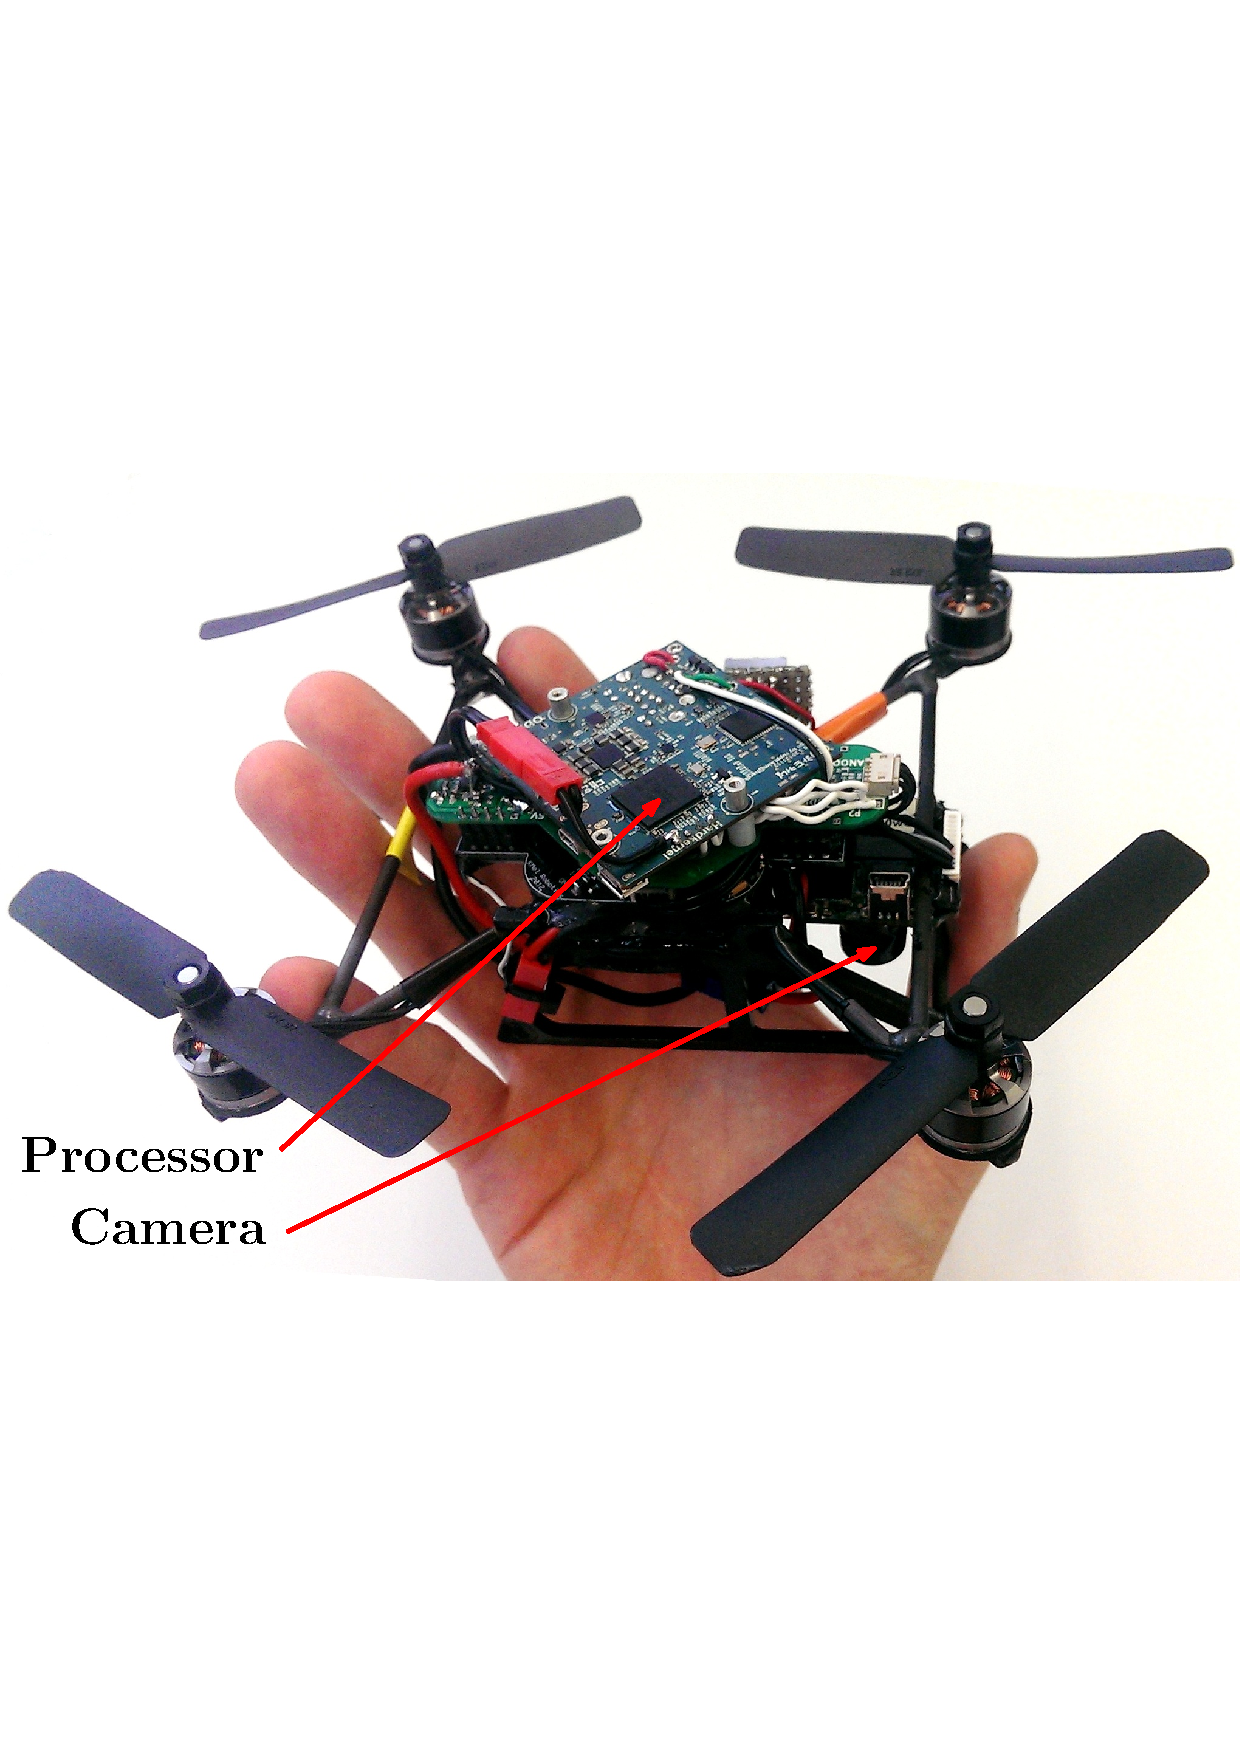
\includegraphics[width=\textwidth]{img/nano}
	  \end{column}
	\end{columns}
\end{frame}

\begin{frame}{Visual Odometry}
	\begin{columns}
	  \begin{column}{0.4\textwidth}
	  	\begin{block}{Problem Formulation}
	  		Two camera poses at adjacent time instants $k-1$ and $k$ are related by the rigid body transformation
	  		\[
				\T_{k,k-1} = \sVec{\mathbf{R} & \mathbf{t} \\ 0 & 0} \in SE(3).
	  		\]
	  		Concatenation of the relative transformations allows to recover the path:
	  		\[
	  			\T_{k,0} = \T_{k,k-1} \cdot \T_{k-1, k-2} \cdots \T_{1, 0}
	  		\]

		\end{block}
	  \end{column}
	  \begin{column}{0.6\textwidth}
	    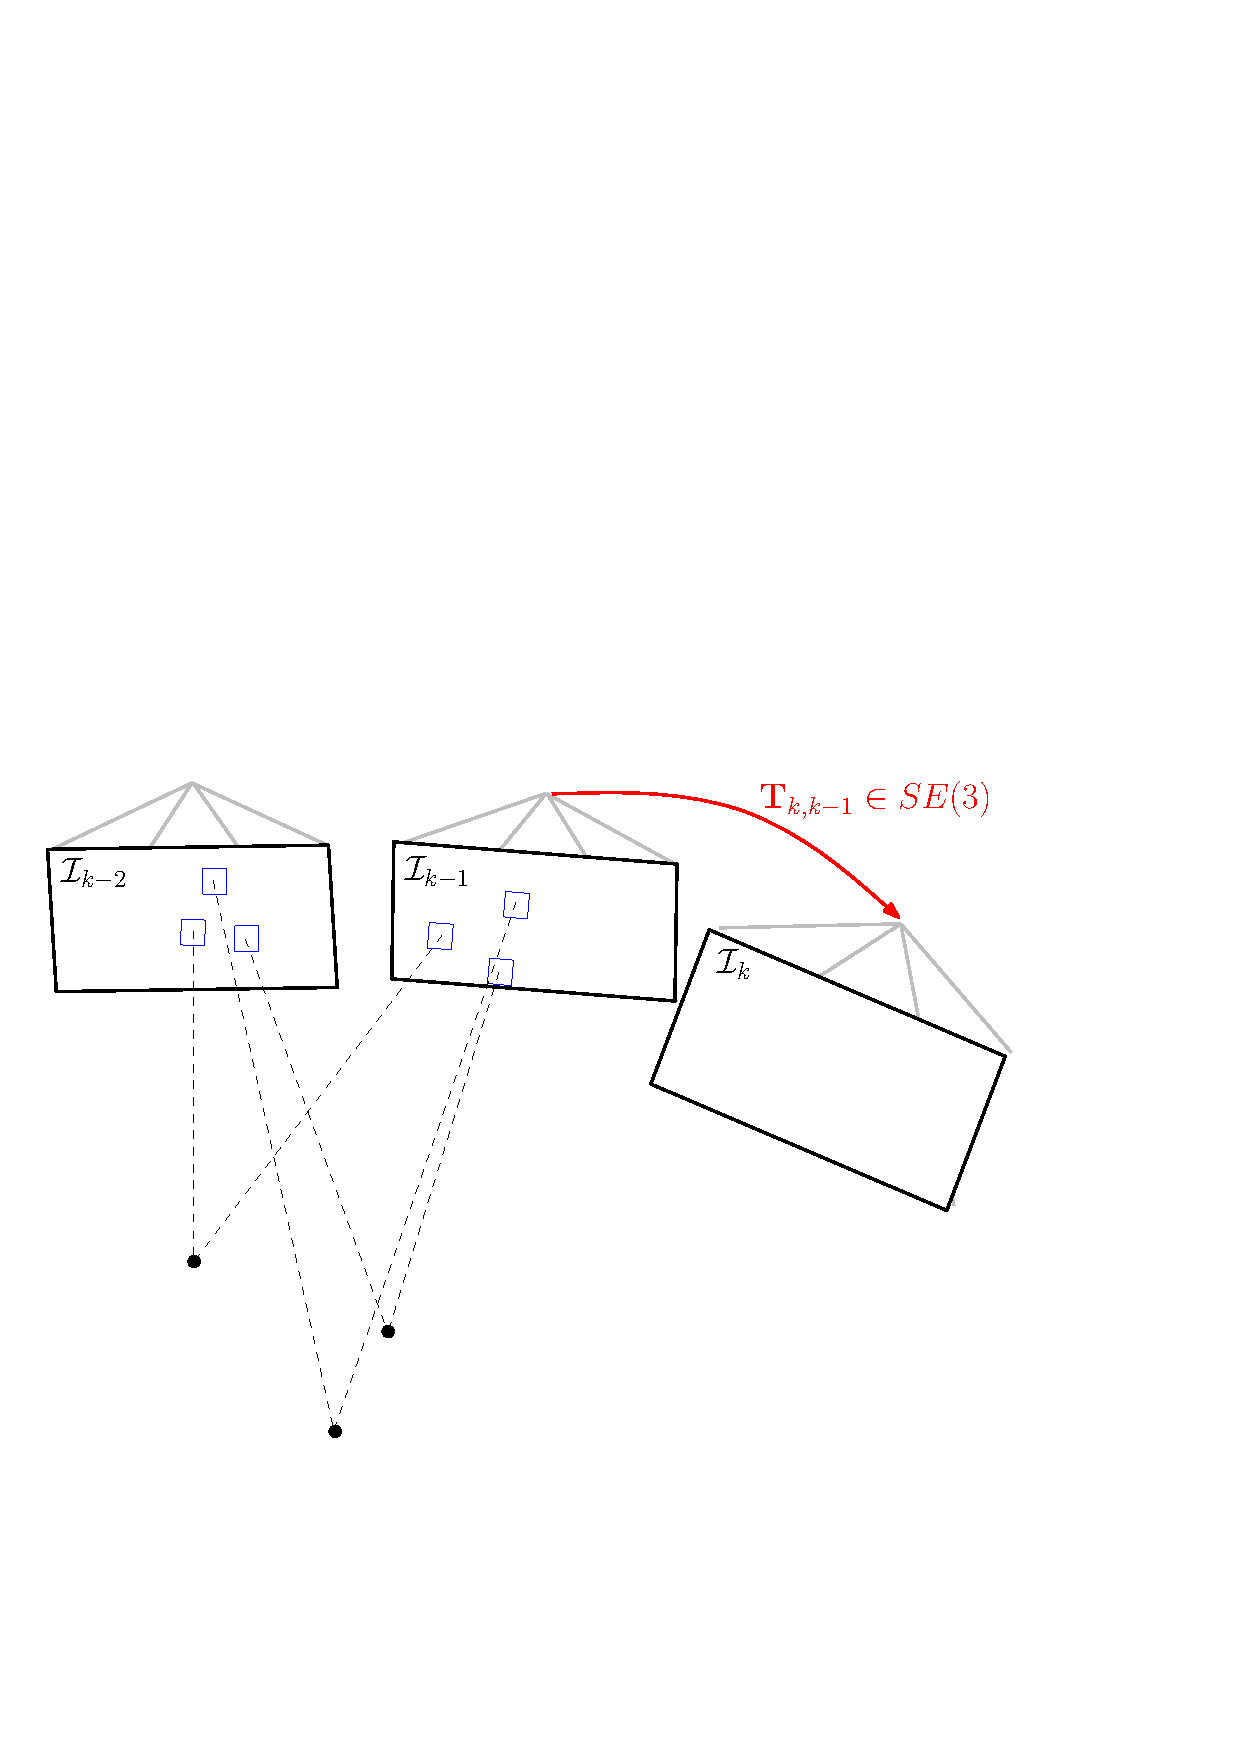
\includegraphics[width=\textwidth]{img/vo_pipeline_2}
	  \end{column}
	\end{columns}
\end{frame}

\begin{frame}{Feature-based Visual Odometry}
	\begin{columns}
	  \begin{column}{0.4\textwidth}
	  	\begin{block}{Pipeline}
		  	\begin{enumerate}
				\item \colorbox{yellow}{Feature selection}
				\item Feature matching 
				\item Pose estimation
				\item Pose refinement
				\item Triangulation
			\end{enumerate}
		\end{block}
		\begin{block}{Which features?}
			\vspace{0.3cm}
			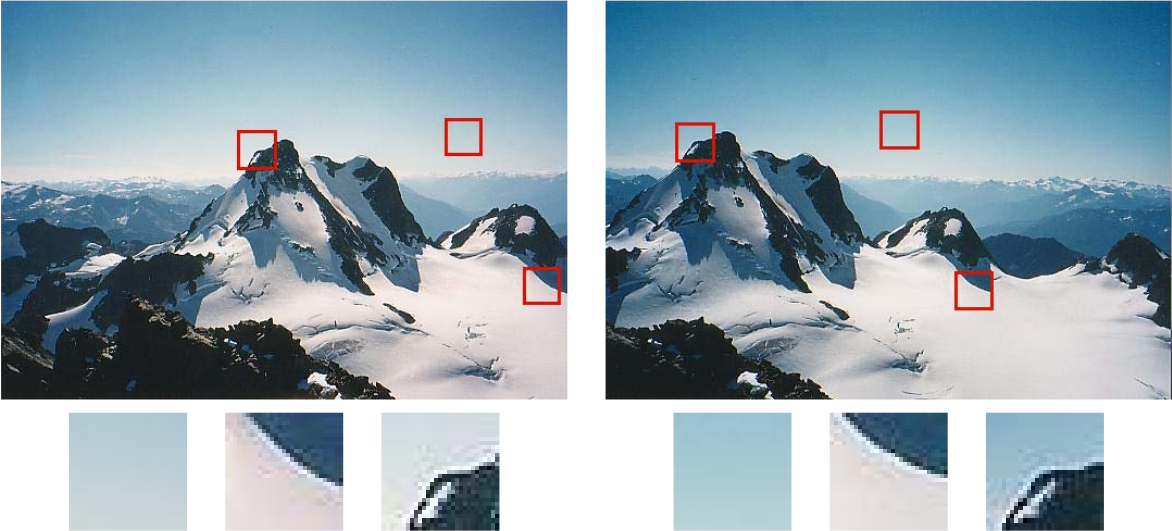
\includegraphics[width=\textwidth]{img/feature_selection.png}
			\vspace{0.1cm}
  			\tiny{\emph{Source: Szeliski, ``Computer Vision: Algorithms and Applications'', Springer 2010.}}
		\end{block}
	  \end{column}
	  \begin{column}{0.6\textwidth}
	    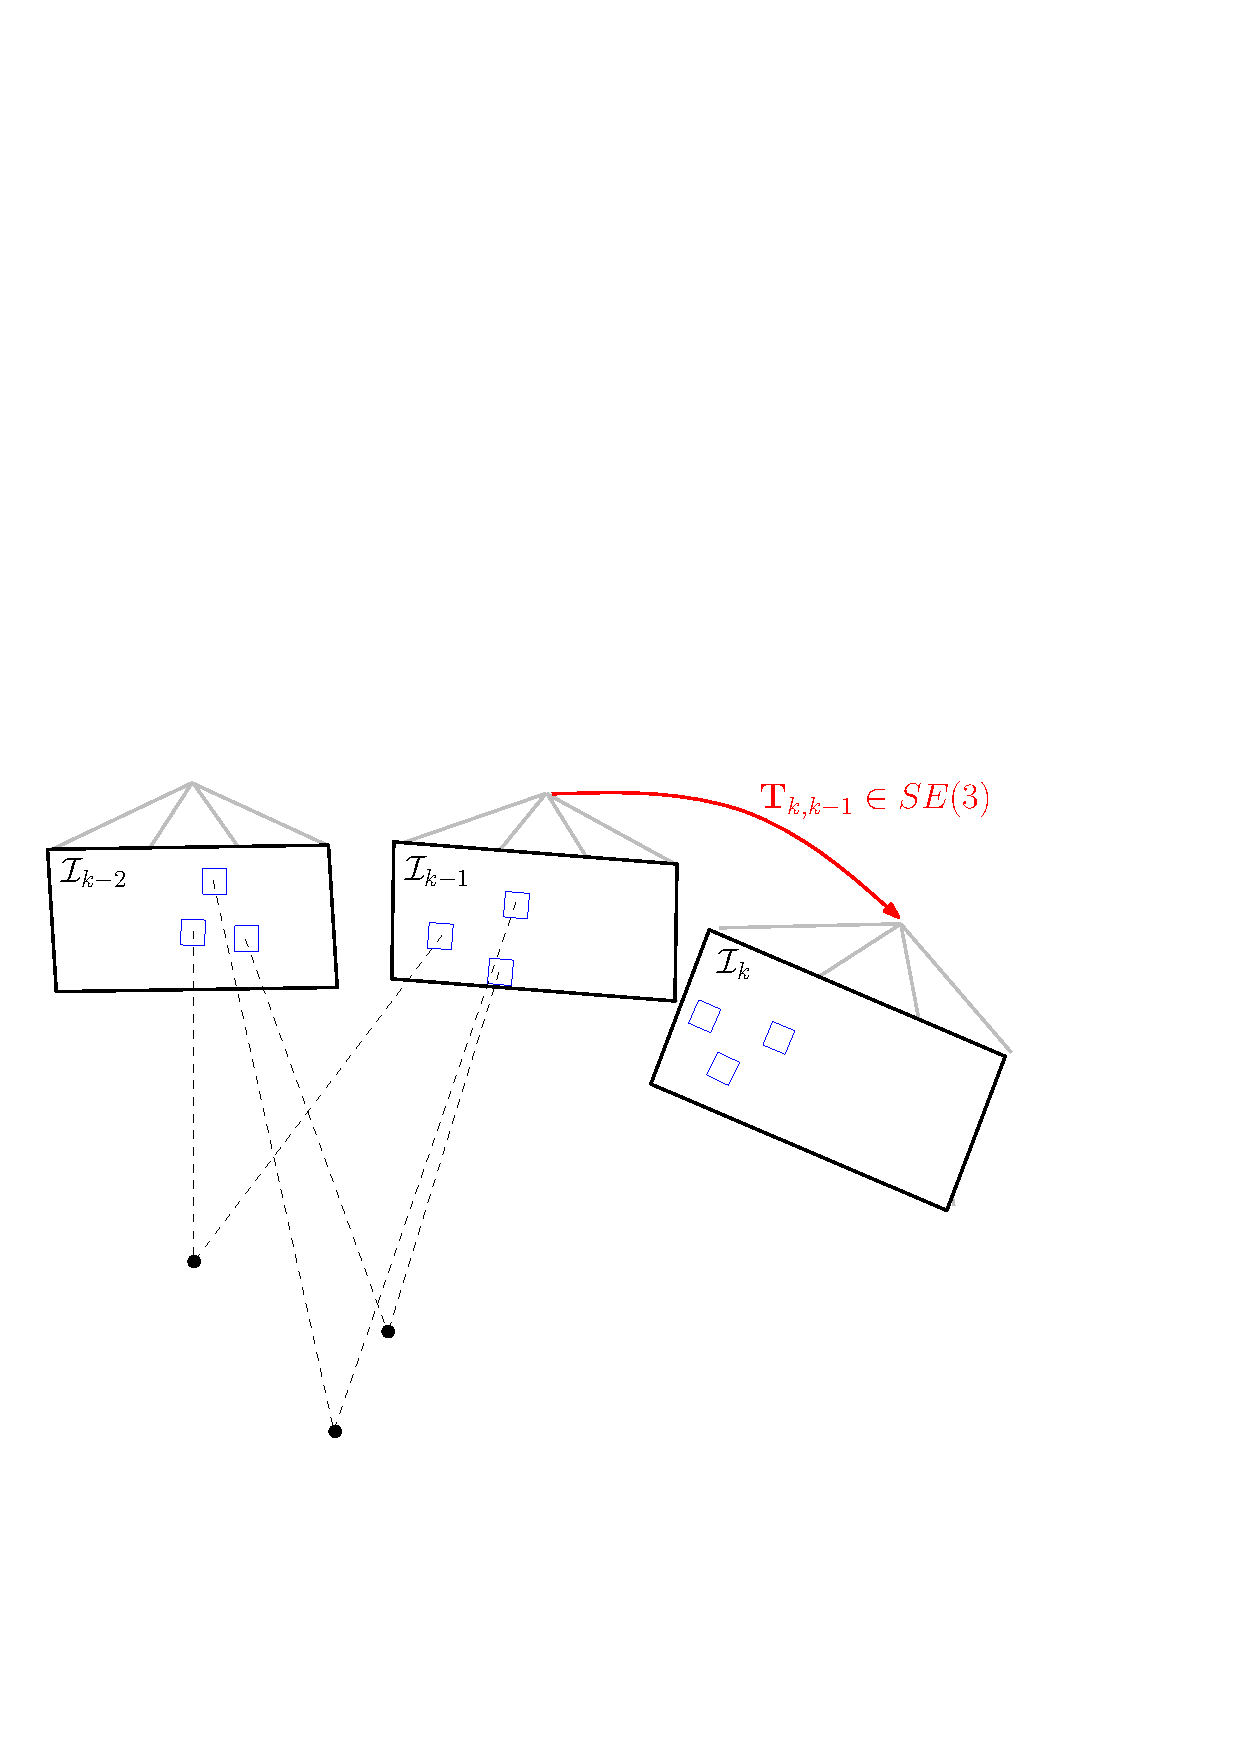
\includegraphics[width=\textwidth]{img/vo_pipeline_3}
	  \end{column}
	\end{columns}
\end{frame}

\begin{frame}{Feature-based Visual Odometry}
	\begin{columns}
	  \begin{column}{0.4\textwidth}
	  	\begin{block}{Pipeline}
		  	\begin{enumerate}
				\item Feature selection
				\item \colorbox{yellow}{Feature matching }
				\item Pose estimation
				\item Pose refinement
				\item Triangulation
			\end{enumerate}
		\end{block}
	  \end{column}
	  \begin{column}{0.6\textwidth}
	    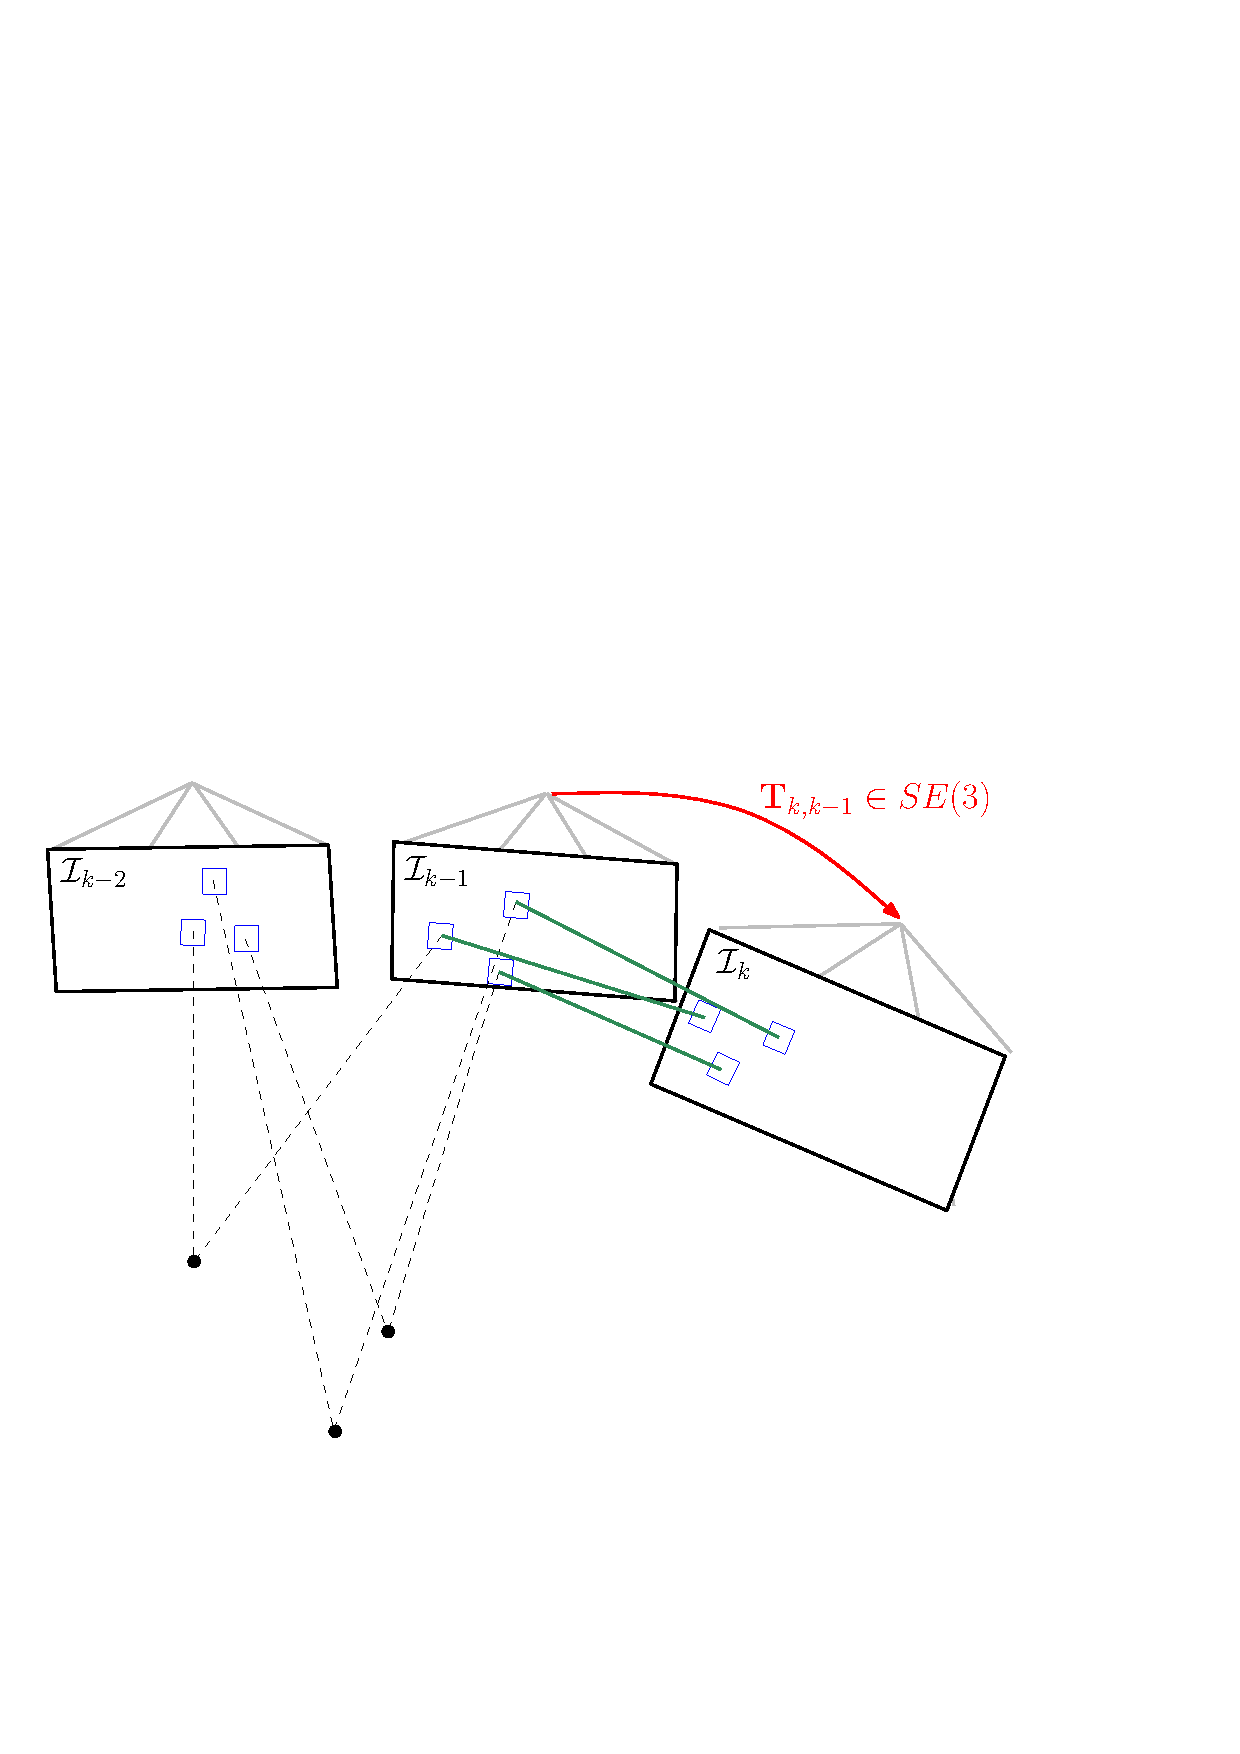
\includegraphics[width=\textwidth]{img/vo_pipeline_4}
	  \end{column}
	\end{columns}
	\begin{columns}
		\begin{column}{0.6\textwidth}
			\begin{block}{Matching Strategies}
				\begin{itemize}
					\item Fast: SSD/NCC over small patch
					\item Robust: Match invariant feature descriptors, e.g., SIFT \mycite{Lowe2003SIFT}
				\end{itemize}
			\end{block}
		\end{column}
		\begin{column}{0.4\textwidth}
		\end{column}
	\end{columns}
\end{frame}

\begin{frame}{Feature-based Visual Odometry}
	\begin{columns}
	  \begin{column}{0.4\textwidth}
	  	\begin{block}{Pipeline}
		  	\begin{enumerate}
				\item Feature selection
				\item Feature matching
				\item \colorbox{yellow}{Pose estimation}
				\item Pose refinement
				\item Triangulation
			\end{enumerate}
		\end{block}
	  \end{column}
	  \begin{column}{0.6\textwidth}
	    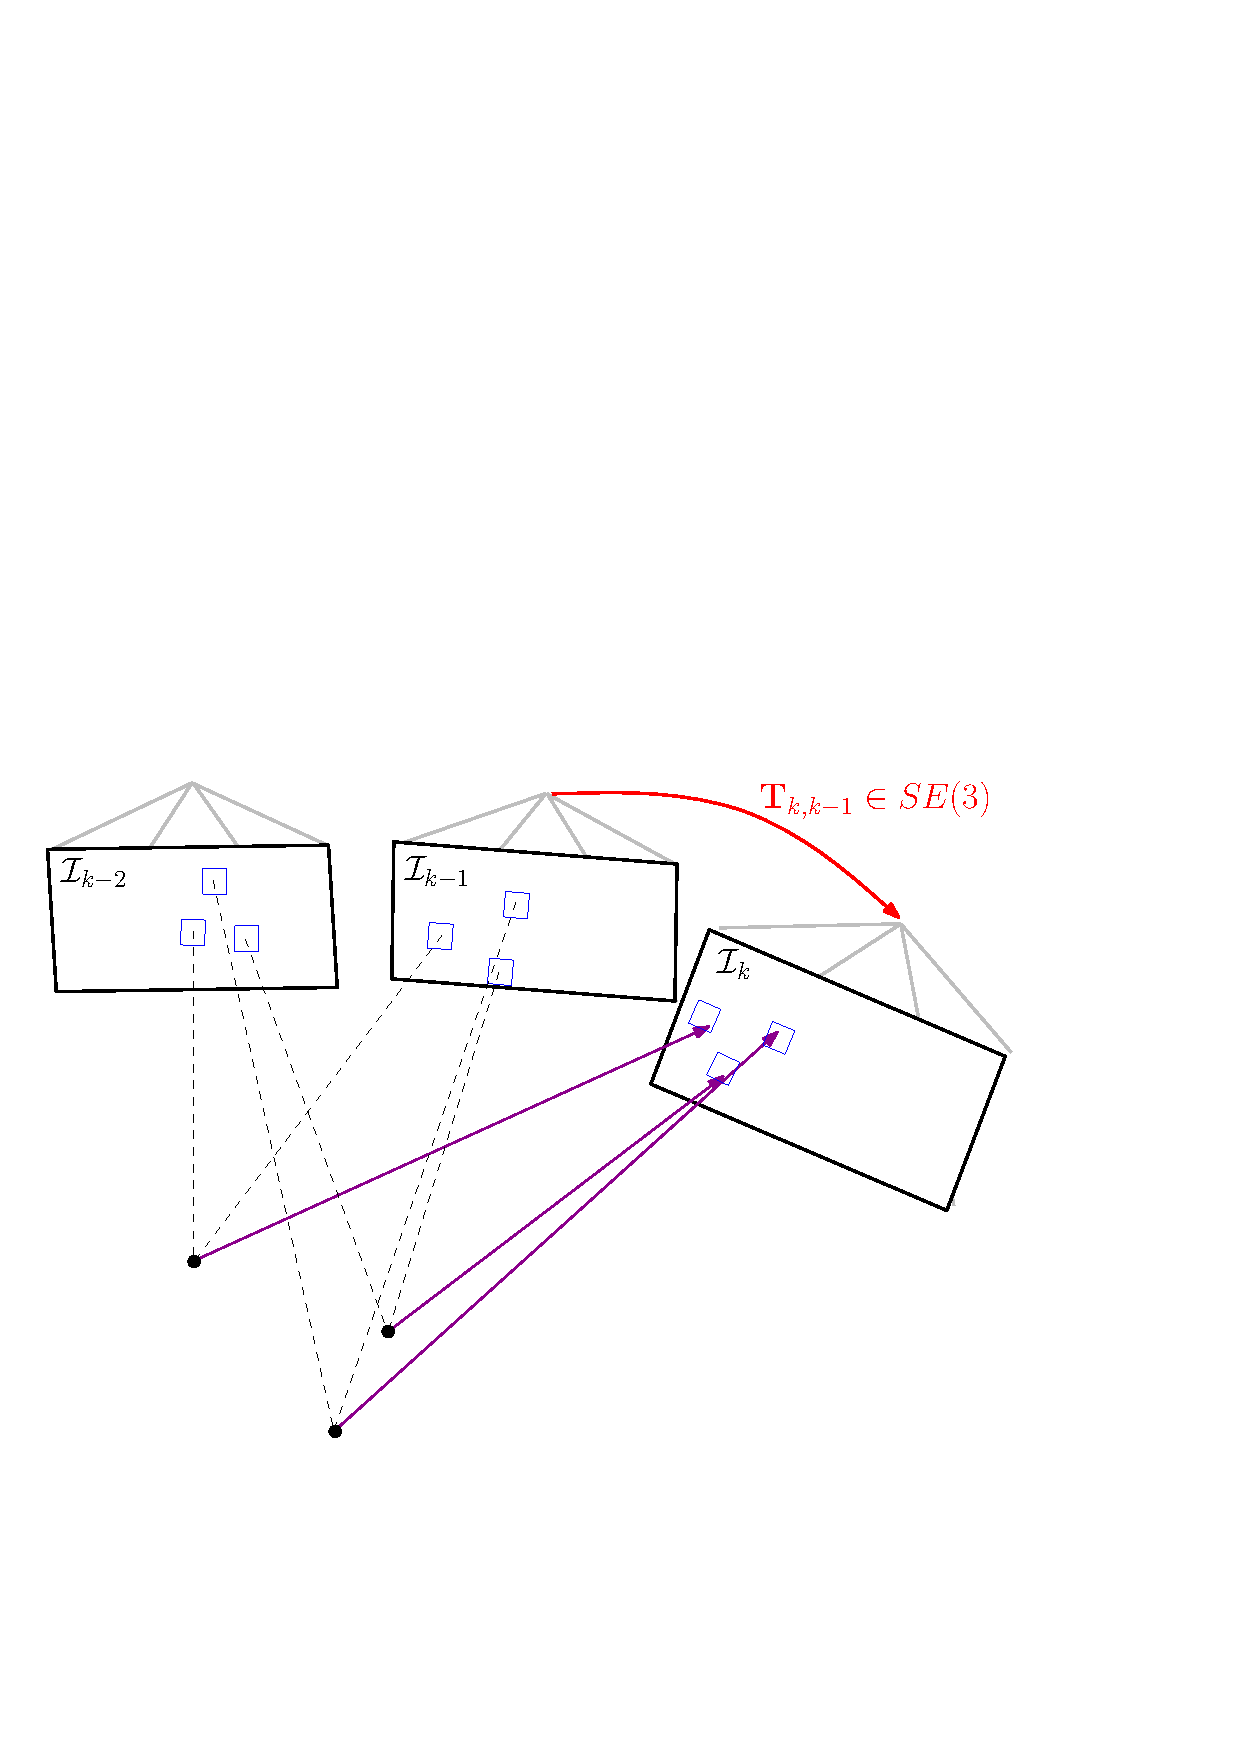
\includegraphics[width=\textwidth]{img/vo_pipeline_5}
	  \end{column}
	\end{columns}
	\begin{columns}
		\begin{column}{0.6\textwidth}
			\begin{block}{Epipolar Geometry}
				Three 3D point to 2D feature correspondences are necessary to estimate the 3D camera pose.
				\mycite{Kneip2011P3P}
			\end{block}
		\end{column}
		\begin{column}{0.4\textwidth}
		\end{column}
	\end{columns}
\end{frame}

\begin{frame}{Feature-based Visual Odometry}
	\begin{columns}
	  \begin{column}{0.4\textwidth}
	  	\begin{block}{Pipeline}
		  	\begin{enumerate}
				\item Feature selection
				\item Feature matching
				\item Pose estimation
				\item \colorbox{yellow}{Pose refinement}
				\item Triangulation
			\end{enumerate}
		\end{block}
		
	  \end{column}
	  \begin{column}{0.6\textwidth}
	    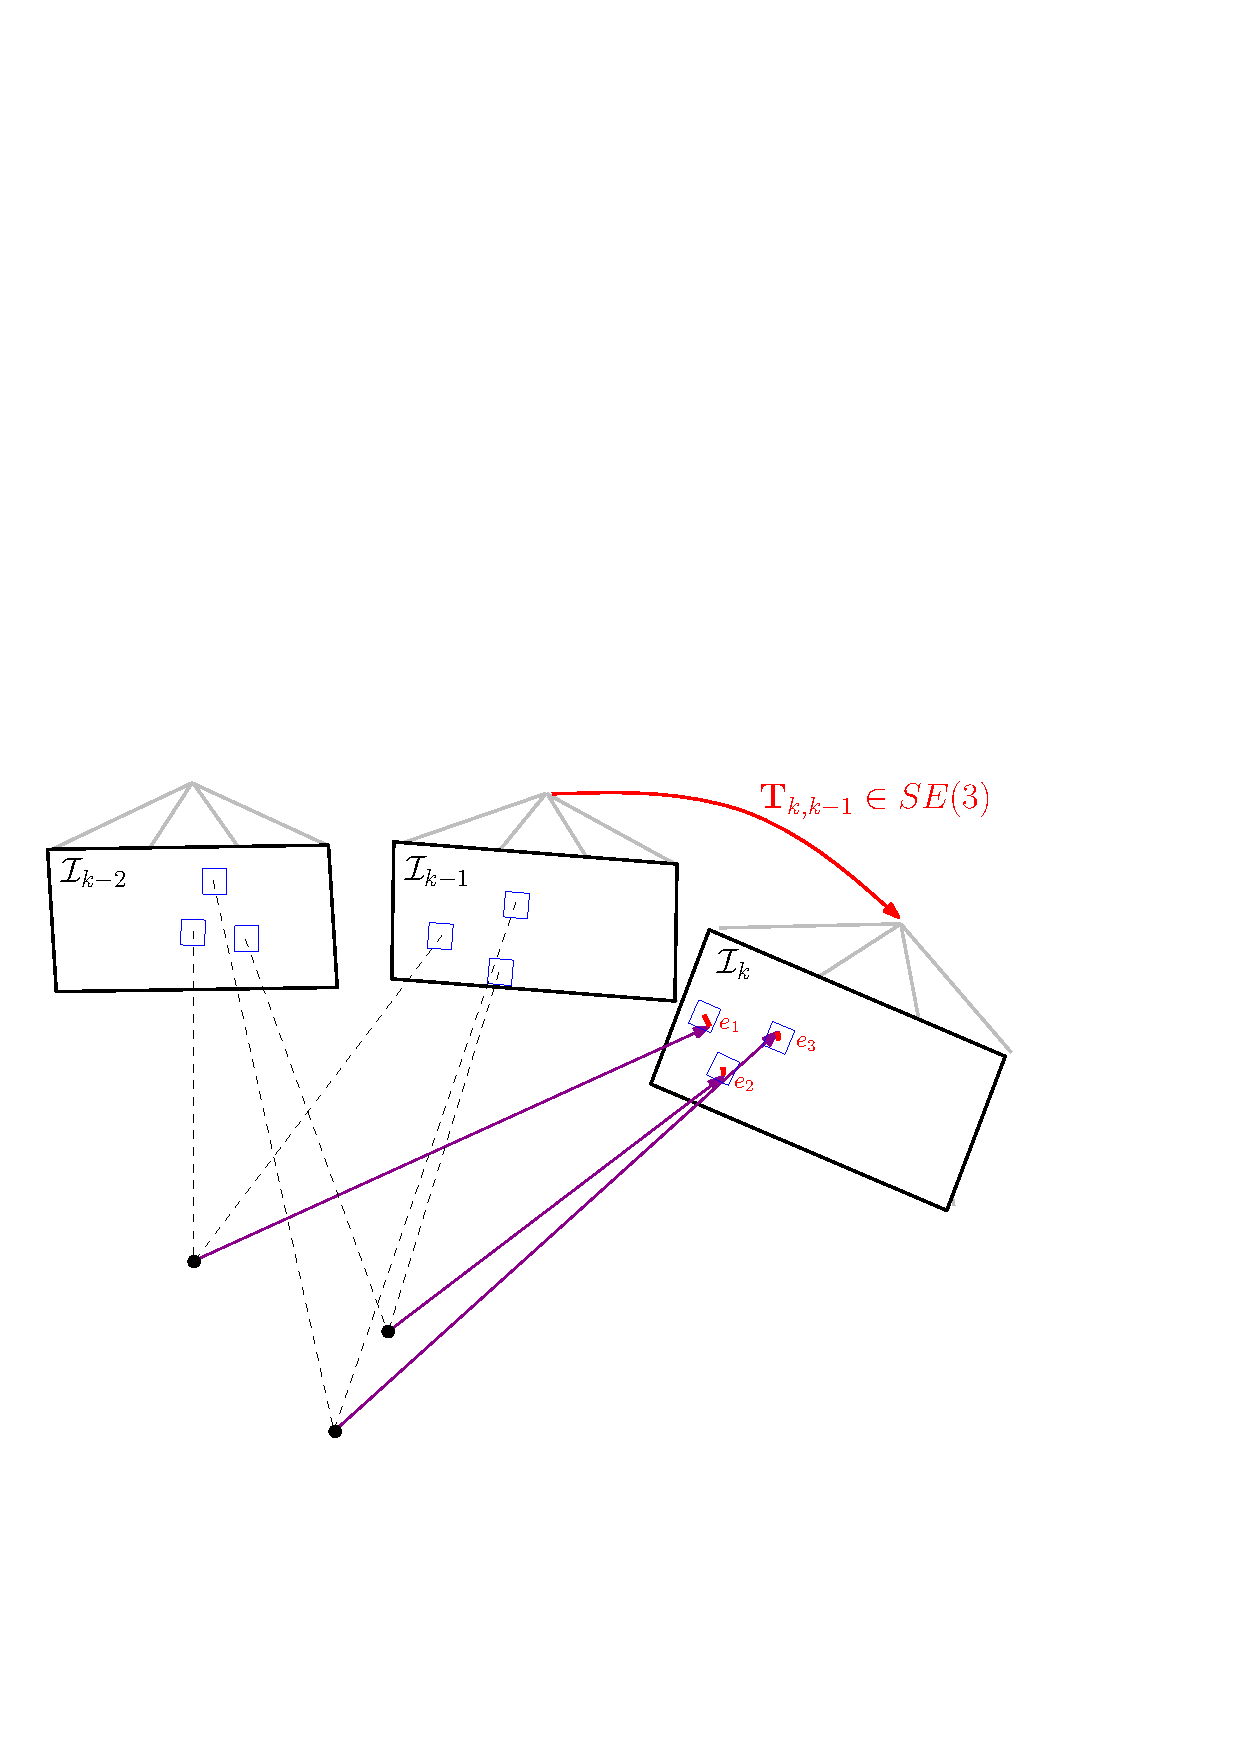
\includegraphics[width=\textwidth]{img/vo_pipeline_6}
	  \end{column}
	\end{columns}
	\begin{columns}
		\begin{column}{0.9\textwidth}
			\begin{block}{Minimize reprojection errors}
				\[
					\T_{k,k-1} = \arg\min_{\T} \sum_{i} \rho \big[ e_i(\T) \big], \qquad \text{typically } \ \rho\big[.\big] \hat{=} \frac{1}{2\sigma^2} \parallel.\parallel^2
				\]
				Can be solved with e.g. Gauss Newton.
			\end{block}
		\end{column}
		\begin{column}{0.1\textwidth}
		\end{column}
    \end{columns}
\end{frame}

\begin{frame}{Feature-based Visual Odometry}
	\begin{columns}
	  \begin{column}{0.4\textwidth}
	  	\begin{block}{Pipeline}
		  	\begin{enumerate}
				\item Feature selection
				\item Feature matching
				\item Pose estimation
				\item Pose refinement
				\item \colorbox{yellow}{Triangulation}
			\end{enumerate}
		\end{block}
		\begin{block}{Triangulation}
			Search along Epipolar line for matching feature.
		\end{block}
	  \end{column}
	  \begin{column}{0.6\textwidth}
	    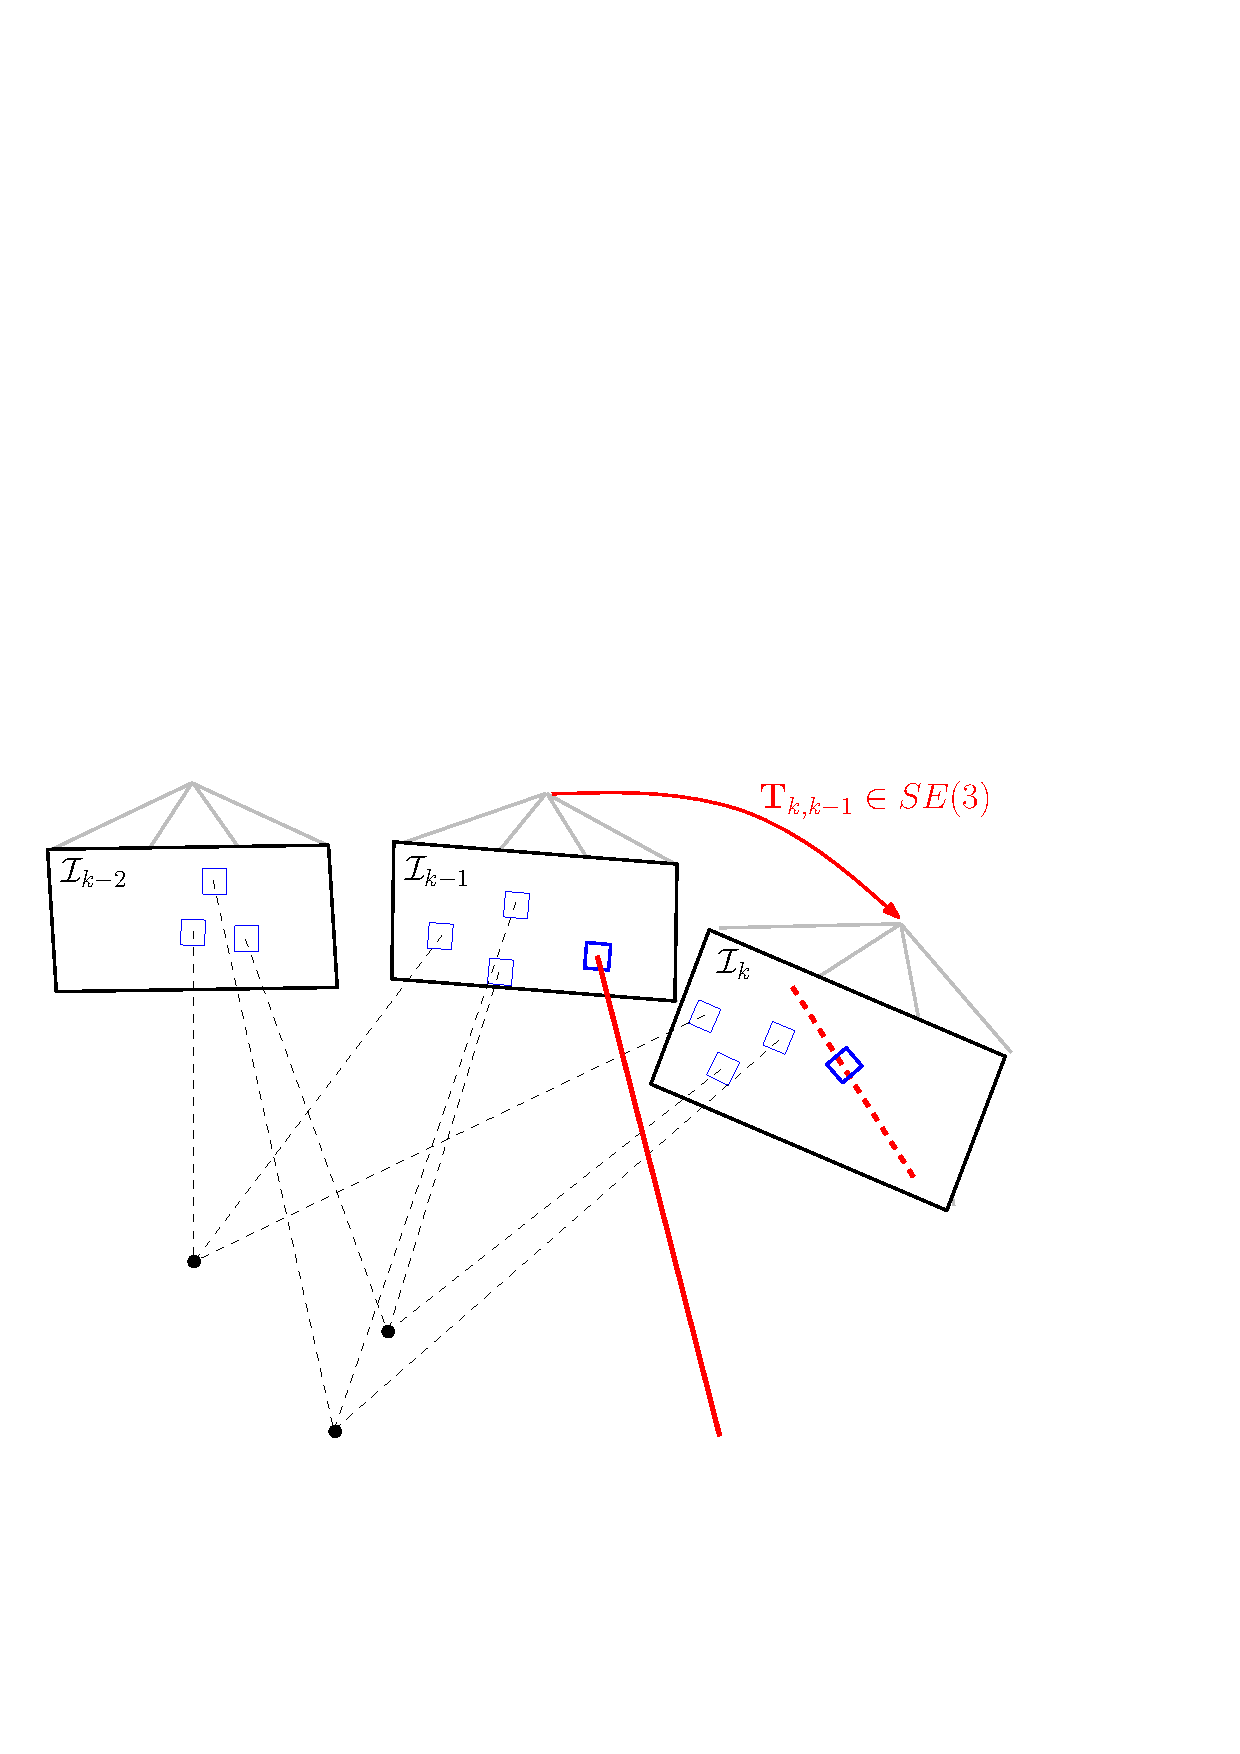
\includegraphics[width=\textwidth]{img/vo_pipeline_7}
	  \end{column}
	\end{columns}
\end{frame}

\begin{frame}{Feature-based Visual Odometry}
	\begin{columns}
	  \begin{column}{0.4\textwidth}
	  	\begin{block}{Pipeline}
		  	\begin{enumerate}
				\item Feature selection
				\item Feature matching
				\item Pose estimation
				\item Pose refinement
				\item \colorbox{yellow}{Triangulation}
			\end{enumerate}
		\end{block}
		\begin{block}{Triangulation}
			Search along Epipolar line for matching feature.
		\end{block}
	  \end{column}
	  \begin{column}{0.6\textwidth}
	    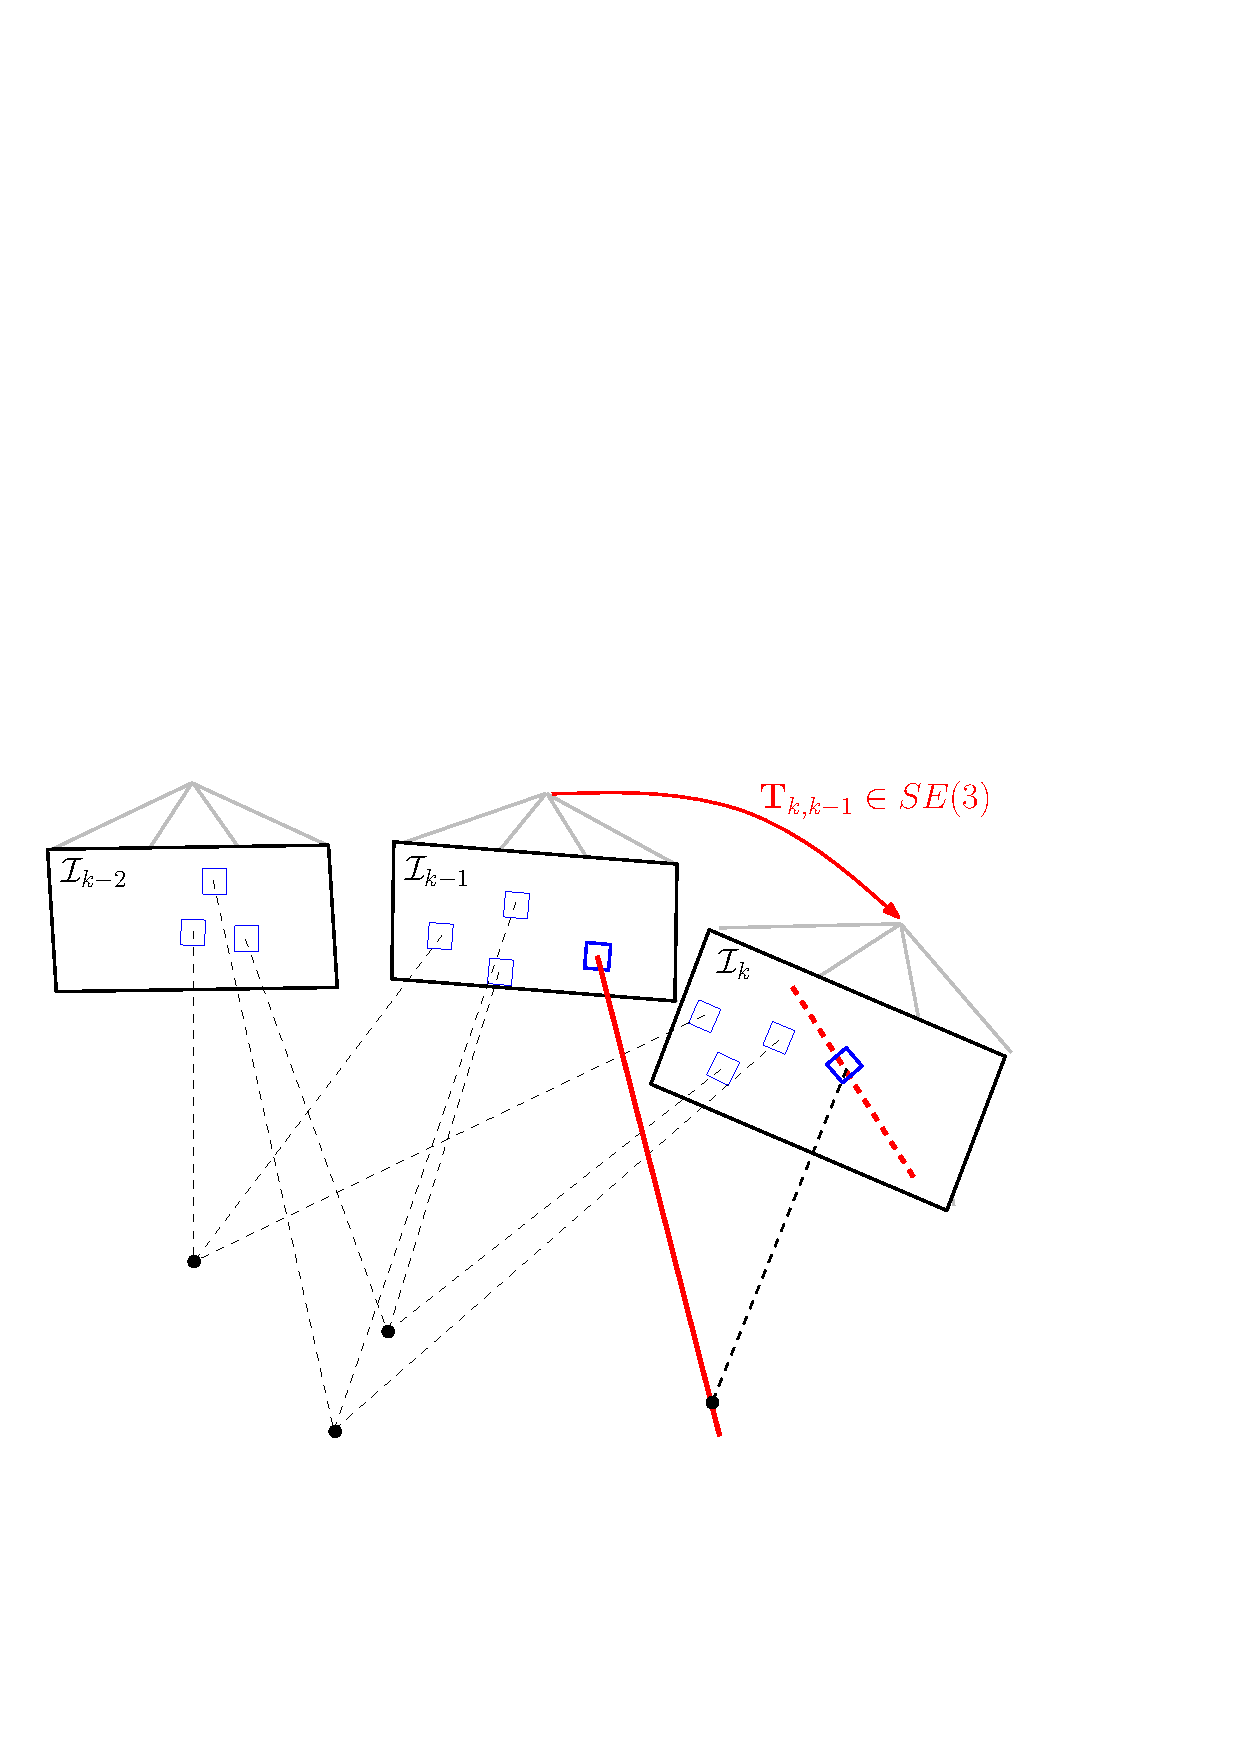
\includegraphics[width=\textwidth]{img/vo_pipeline_8}
	  \end{column}
	\end{columns}
\end{frame}

\begin{frame}{Implementation Details}
	\begin{itemize}
		\item Make more robust by using many (hundreds) of features.
		\item Use motion model to speed-up feature matching.
		\item Use robust estimation techniques to handle wrong matches (e.g., RANSAC \mycite{FischlerBolles1981}).
		\item Minimize drift through incremental Bundle Adjustment: Joint optimization of frames and 3D points \mycite{Mouragnon2006}.
		\item Parallelize tracking and mapping \mycite{Klein2009}.
	\end{itemize}
\end{frame}


\begin{frame}{The direct approach}
	\begin{columns}
	  	\begin{column}{0.5\textwidth}
	  		\begin{block}{Minimize photometric error}
			  	\[
		  			\T_{k,k-1} = \arg\min_\T \iint_{\bar{\mathcal{R}}} \rho\Big[ \delta \I\big(\T, \bu\big) \Big] d\bu.
				\]
				where
				\[ 
					\begin{aligned}
				  		\delta \I\big(\T, \bu\big) &= \I_k(\bu') - \I_{k-1}(\bu) \\
				  		\bu' &= \pi\big(\T \cdot \pi^{-1}(\bu, z_\bu)\big) 
			   		\end{aligned}
				\]
			\end{block}
		\end{column}
	    \begin{column}{0.5\textwidth}
		    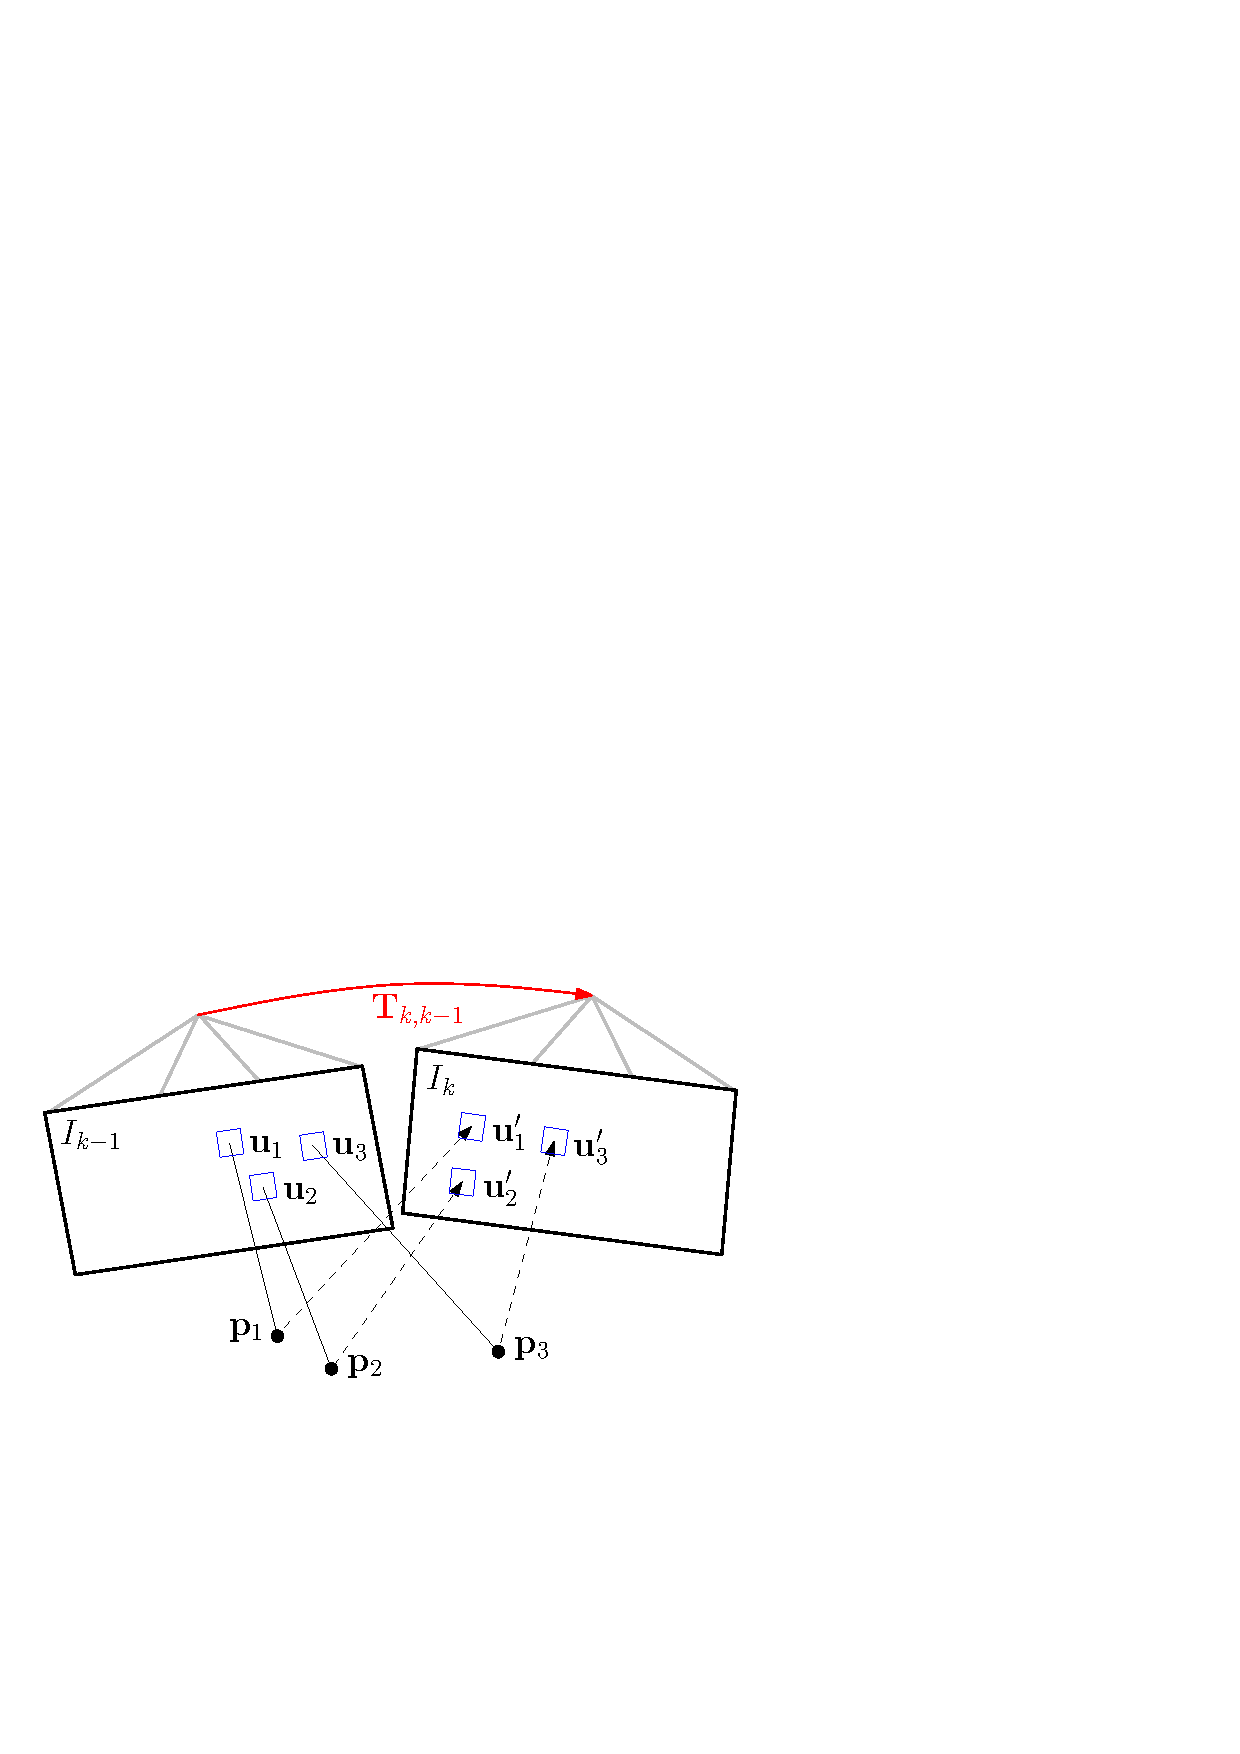
\includegraphics[width=\textwidth]{img/sparse_img_alignment}
		\end{column}
	\end{columns}
	\begin{columns}
		\begin{column}{0.9\textwidth}
			\begin{block}{Advantages}
				\begin{itemize}
					\item No costly feature extraction
					\item No costly robust feature matching
				\end{itemize}
			\end{block}
			\mycite{Forster2014NSLAM}
		\end{column}
		\begin{column}{0.1\textwidth}
		\end{column}
	\end{columns}	
\end{frame}

\begin{frame}{Future Challenges}
	\begin{columns}
		\begin{column}{0.5\textwidth}
			\begin{itemize}
				\item Robust performance in scenes of little, repetitive or high frequency texture.
				\item Robust tracking under disturbances: Moving objects, changing light conditions.
				\item Fast relocalization after tracking failure.
			\end{itemize}
		\end{column}
	    \begin{column}{0.5\textwidth}
		    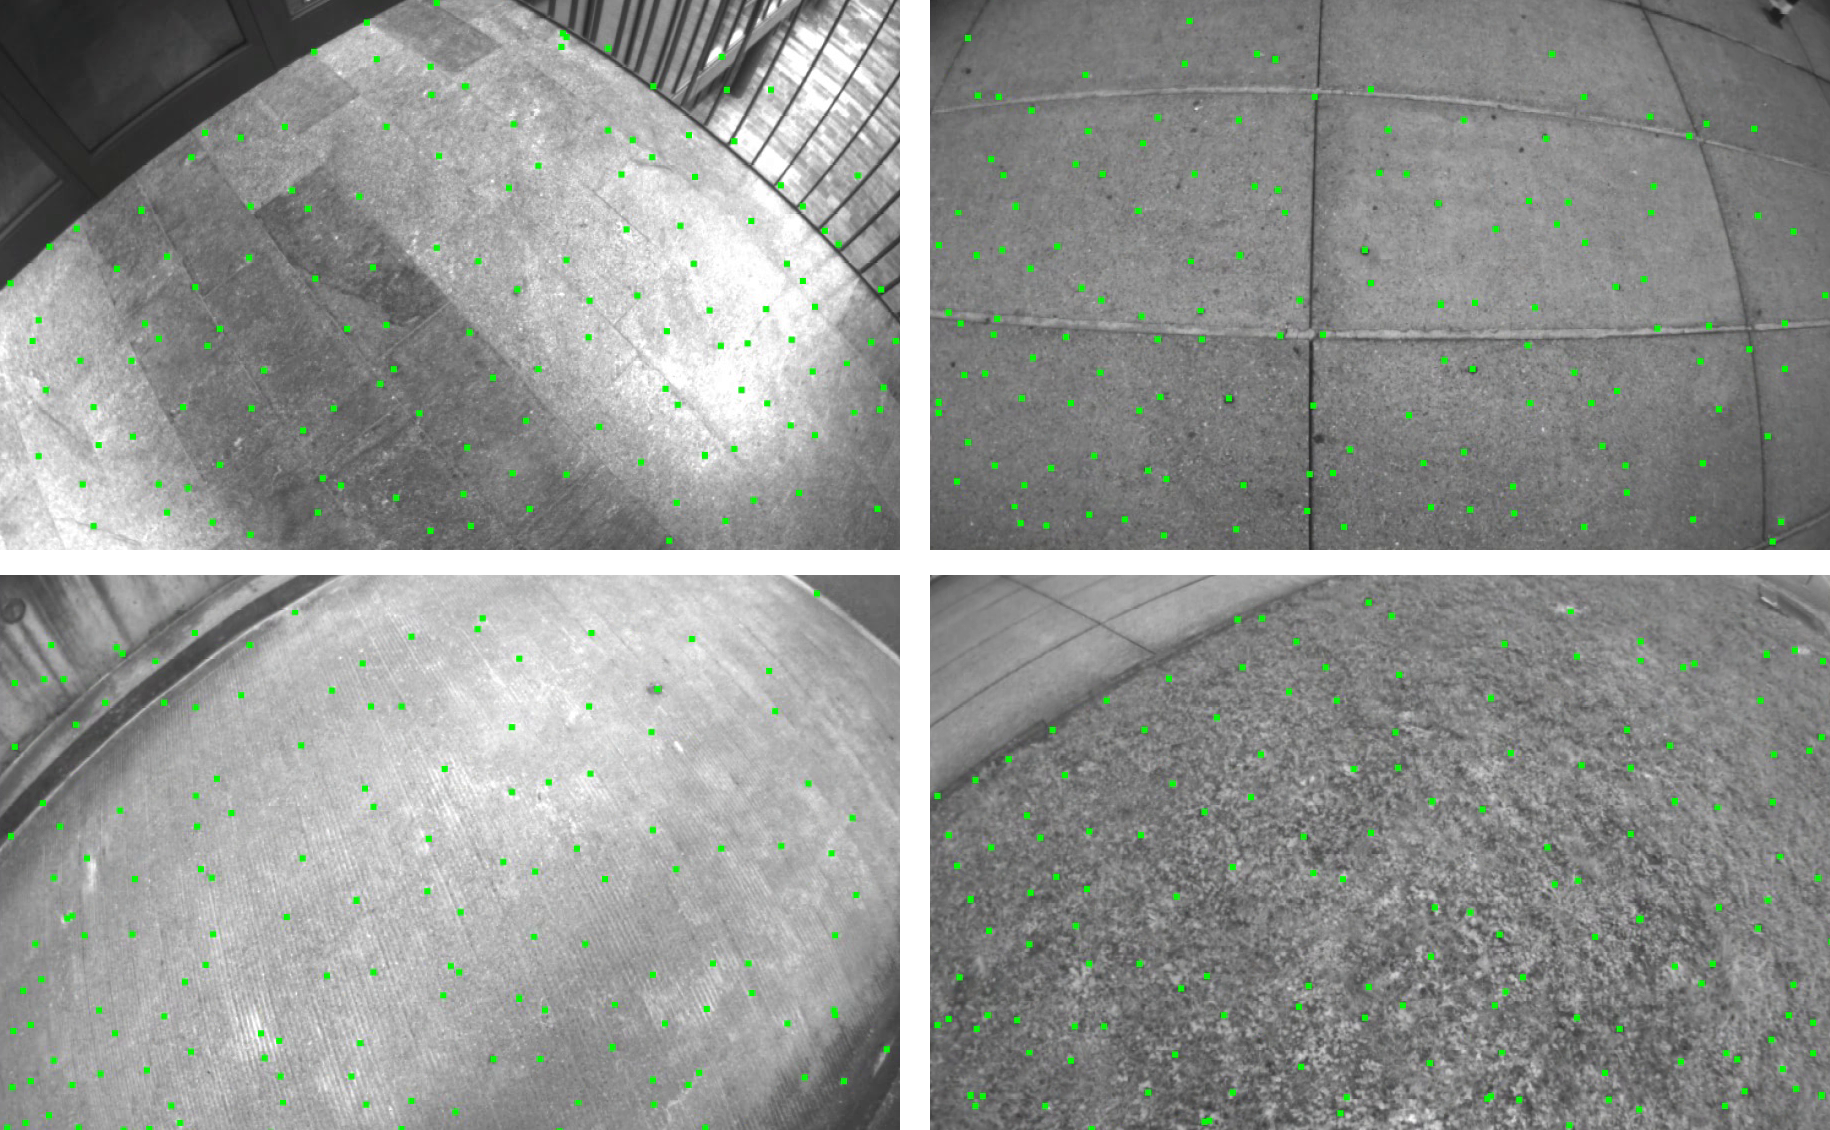
\includegraphics[width=\textwidth]{img/tracking_performance.png}\\
		    \footnotesize{\emph{High frequency texture}}\\
		    \vspace{0.3cm}
		    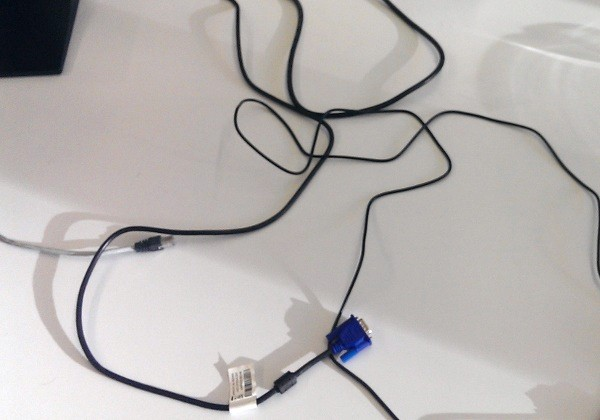
\includegraphics[width=\textwidth]{img/no_corners.jpg}\\
		    \footnotesize{\emph{No corners}}
		\end{column}
	\end{columns}	
\end{frame}

\begin{frame}{Bibliography}
	\bibliographystyle{apalike}
	\bibliography{bibliography}
\end{frame}

\end{document}